\documentclass[15pt,a5paper,reqno]{article}
\usepackage{hyperref}
\usepackage[warn]{mathtext}
\usepackage[utf8x]{inputenc}
\usepackage{amssymb, amsmath, multicol}
\usepackage[russian]{babel}
\usepackage{graphicx}
\usepackage[shortcuts,cyremdash]{extdash}
\usepackage{wrapfig}
\usepackage{floatflt}
\usepackage{lipsum}
\usepackage{verbatim}
\usepackage{concmath}
\usepackage{euler}
\usepackage{xcolor}
\usepackage{etoolbox}
\usepackage{fancyhdr}
\usepackage{subfiles}
\usepackage{enumitem}
\usepackage{amsthm}
\usepackage{indentfirst}
\usepackage{import}

\DeclareMathOperator{\sign}{sign}

\RequirePackage[ left     = 1.5cm,
  right    = 1.5cm,
  top      = 2.0cm,
  bottom   = 1.25cm,
  includefoot,
  footskip = 1.25cm ]{geometry}
\setlength    {\parskip}        { .5em plus .15em minus .08em }
%\setlength    {\parindent}      { .0em }
\renewcommand {\baselinestretch}{ 1.07 }

\fancyhf{}

\renewcommand{\footrulewidth}{ .0em }
\fancyfoot[C]{\texttt{\textemdash~\thepage~\textemdash}}
\fancyhead[R]{\hfilШурыгин}

\makeatletter
\patchcmd\l@section{%
  \nobreak\hfil\nobreak
}{%
  \nobreak
  \leaders\hbox{%
    $\m@th \mkern \@dotsep mu\hbox{.}\mkern \@dotsep mu$%
  }%
  \hfill
  \nobreak
}{}{\errmessage{\noexpand\l@section could not be patched}}
\makeatother
\parindent = 1cm % отступ при красной строке⏎
\pagestyle{fancy}    
\renewcommand\qedsymbol{$\blacksquare$}

\newcommand{\when}[2]{
  \left. #1 \right|_{#2} \hspace
}
\renewcommand{\kappa}{\varkappa}
\RequirePackage{caption2}
\renewcommand\captionlabeldelim{}
\newcommand*{\hm}[1]{#1\nobreak\discretionary{}

\DeclareSymbolFont{T2Aletters}{T2A}{cmr}{m}{it}
{\hbox{$\mathsurround=0pt #1$}}{}}
% Цвета для гиперссылок
\definecolor{linkcolor}{HTML}{000000} % цвет ссылок
\definecolor{urlcolor}{HTML}{799B03} % цвет гиперссылок
 
\hypersetup{pdfstartview=FitH,  linkcolor=linkcolor,urlcolor=urlcolor, colorlinks=true}


%\setcounter{secnum[utf8x]depth}{0}

\begin{document}

% НАЧАЛО ТИТУЛЬНОГО ЛИСТА
\begin{center}
  {\small ФЕДЕРАЛЬНОЕ ГОСУДАРСТВЕННОЕ АВТОНОМНОЕ ОБРАЗОВАТЕЛЬНОЕ\\ УЧРЕЖДЕНИЕ ВЫСШЕГО ОБРАЗОВАНИЯ\\ МОСКОВСКИЙ ФИЗИКО-ТЕХНИЧЕСКИЙ ИНСТИТУТ\\ (НАЦИОНАЛЬНЫЙ ИССЛЕДОВАТЕЛЬСКИЙ УНИВЕРСИТЕТ)\\ ФИЗТЕХ-ШКОЛА РАДИОТЕХНИКИ И КИБЕРНЕТИКИ}\\
  \hfill \break
  \hfill \break
  \hfill \break
  \Huge{Дифракция света.}\\
\end{center}

\hfill \break
\hfill \break
\hfill \break
\hfill \break
\hfill \break
\hfill \break

\begin{flushright}
  \normalsize{Работу выполнил:}\\
  \normalsize{\textbf{Шурыгин Антон Алексеевич, группа Б01-909}}\\
\end{flushright}

\begin{center}
  \normalsize{\textbf{Долгопрудный, 2021}}
\end{center}


\thispagestyle{empty} % выключаем отображение номера для этой страницы

% КОНЕЦ ТИТУЛЬНОГО ЛИСТА

\newpage
\thispagestyle{plain}
\tableofcontents
\thispagestyle{plain}
\newpage


	\paragraph*{Цель работы:} исследовать явления дифракции Френеля и Фраунгофера на щели, изучить влияние дифракции на разрешающую способность оптических инструментов.
	
	\paragraph*{Оборудование:} оптическая скамья, ртутная лампа, монохроматор, щели с регулируемой шириной, рамка с вертикальной
нитью, двойная щель, микроскоп на поперечных салазках с микрометрическим винтом, зрительная труба.

	\section{Дифракция Френеля}
	
	\subsection{Экспериментальная установка}
	
	Схема установки для наблюдения дифракции Френеля на щели
представлена на рис. 1. Световые лучи освещают щель $ S_2 $ и испытывают на ней дифракцию. Дифракционная картина рассматривается с помощью микроскопа М, сфокусированного на некоторую плоскость наблюдения П.
	
	\begin{figure}[h!]
		\centering
		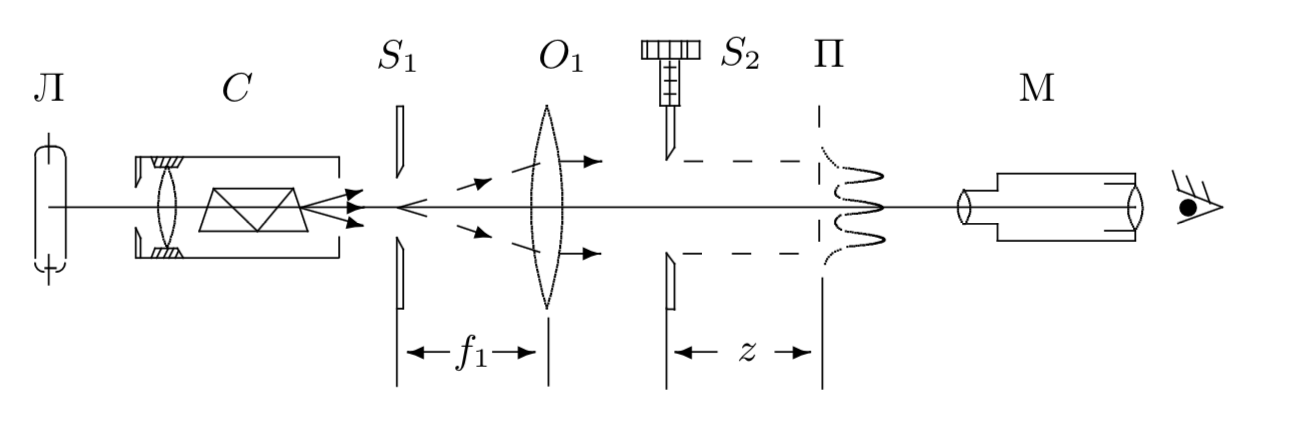
\includegraphics[width=0.8\linewidth]{pics/a.png}
		\caption{Экспериментальная установка A}
		\label{labA}
	\end{figure}

Щель $ S_2 $ освещается параллельным пучком монохроматического
света с помощью коллиматора, образованного объективом $ O_1 $, и ще-
лью S1, находящейся в его фокусе. На щель $ S_1 $ сфокусировано изображение спектральной линии, выделенной из спектра ртутной лампы Л
при помощи простого монохроматора C, в котором используется приз-
ма прямого зрения.
Распределение интенсивности света в плоскости наблюдения П про-
ще всего рассчитывать с помощью зон Френеля (для щели их иногда
называют зонами Шустера). При освещении щели $ S_2 $ параллельным пучком лучей (плоская волна) зоны Френеля представляют собой по-
лоски, параллельные краям щели (рис. 2). Результирующая амплитуда
в точке наблюдения определяется суперпозицией колебаний от тех зон
Френеля, которые не перекрыты створками щели. Графическое определение результирующей амплитуды производится с помощью векторной
диаграммы --- спирали Корню. Суммарная ширина $ n $ зон Френеля (Шустера) определяется соотношением:

\begin{equation}\label{xin}
\xi_n = \sqrt{zn\lambda}
\end{equation}

где $ z $ --- расстояние от щели до плоскости наблюдения (рис. 1), а $ \lambda $ --- длина волны.

\begin{wrapfigure}{r}{0.35\linewidth} 
	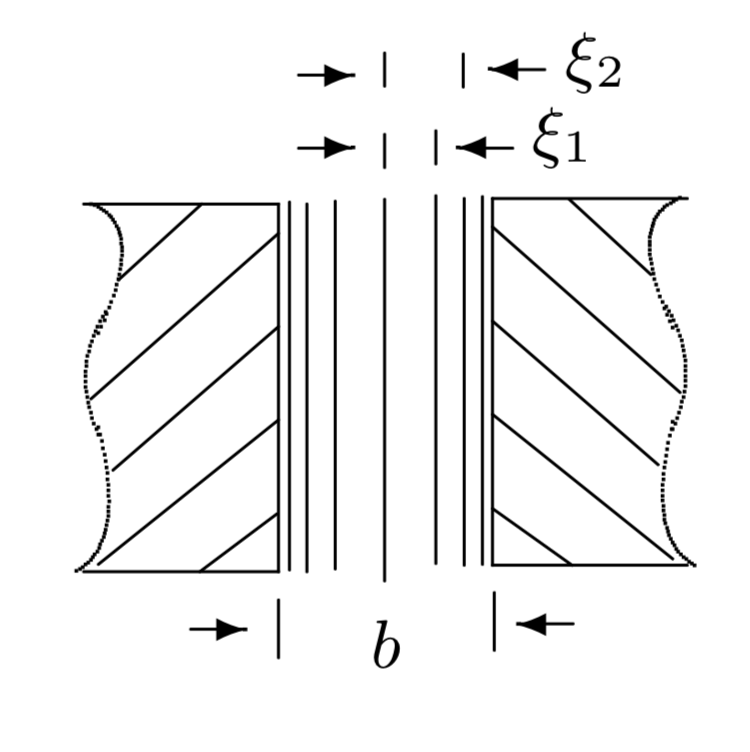
\includegraphics[width=\linewidth]{pics/zone}
	\caption{Зоны Френеля}
	\label{zone}
\end{wrapfigure}

Вид наблюдаемой дифракционной картины
на щели шириной $ b $ определяется волновым параметром $ p $ или числом Френеля $ C $ (число открытых полных зон):


\begin{equation}\label{}
p = \dfrac{\sqrt{z \lambda}}{b}, \qquad C = \dfrac{1}{p^2}
\end{equation}

Дифракционная картина отсутствует вблизи щели при $ p \ll 1 $
($ C \gg 1 $, т. е. на щели укладывается огромное число зон), а распределение интенсивности света за щелью можно приближённо получить
с помощью законов геометрической оптики. Дифракционная картина
в этом случае наблюдается только в узкой области на границе света и
тени у краёв экрана.

При небольшом удалении от щели (или изменении ширины щели $ S_2 $) эти две группы дифракционных полос перемещаются практически независимо друг от друга. Каждая из этих групп образует картину дифракции Френеля на краю экрана. Распределение интенсивности
при дифракции света на краю экрана может быть найдено с помощью
спирали Корню.

При дальнейшем увеличении расстояния $ z $ (или уменьшении шири-
ны щели $ S_2 $) обе системы дифракционных полос постепенно сближаются и, наконец, при $ C \gtrsim 1 $ накладываются друг на друга. Распределение интенсивности в плоскости наблюдения в этом случае определяется
числом зон Френеля, укладывающихся на полуширине щели $ b/2 $. Если это число равно $ n $, то в поле зрения наблюдается $ m = n - 1 $ тёмных полос. Таким образом, по виду дифракционной картины можно оценить
число зон Френеля на полуширине щели.

\subsection{Измерения и обработка результатов}

Запишем ширину щели: $ b = 0,200 \pm 0,005 $ мм. 

Приближая микроскоп к щели, снимем зависимость координаты $z $ мм микроскопа от числа $ n $ темных полос.
\newline
Результаты занесем в табл. 1 и построим график зависимости величины $ 2\xi_n $ (формула \eqref{xin}) от $ n $. Длина волны зеленого света $ \lambda = 5461 \cdot 10^{-10} $ м. 

\begin{table}[h!]
\caption{Зависимость координаты микроскопа от числа $ n $ темных полос}
\begin{center}
	\begin{tabular}{|c|c|c|}
		\hline
		$ n $ & $ z $, мм & $ 2\xi_n $, мм\\
		\hline
		1 & 10 & 0.147 \\
	    \hline
		2 & 7 & 0.174 \\
		\hline
		3 & 5 & 0.181 \\
		\hline
		4 & 4.5 & 0.198 \\
		\hline
		5 & 4 & 0.209 \\
		\hline
	\end{tabular}
\end{center}
\label{}
\end{table}

\begin{figure}[h!]
	\label{graf_a}
	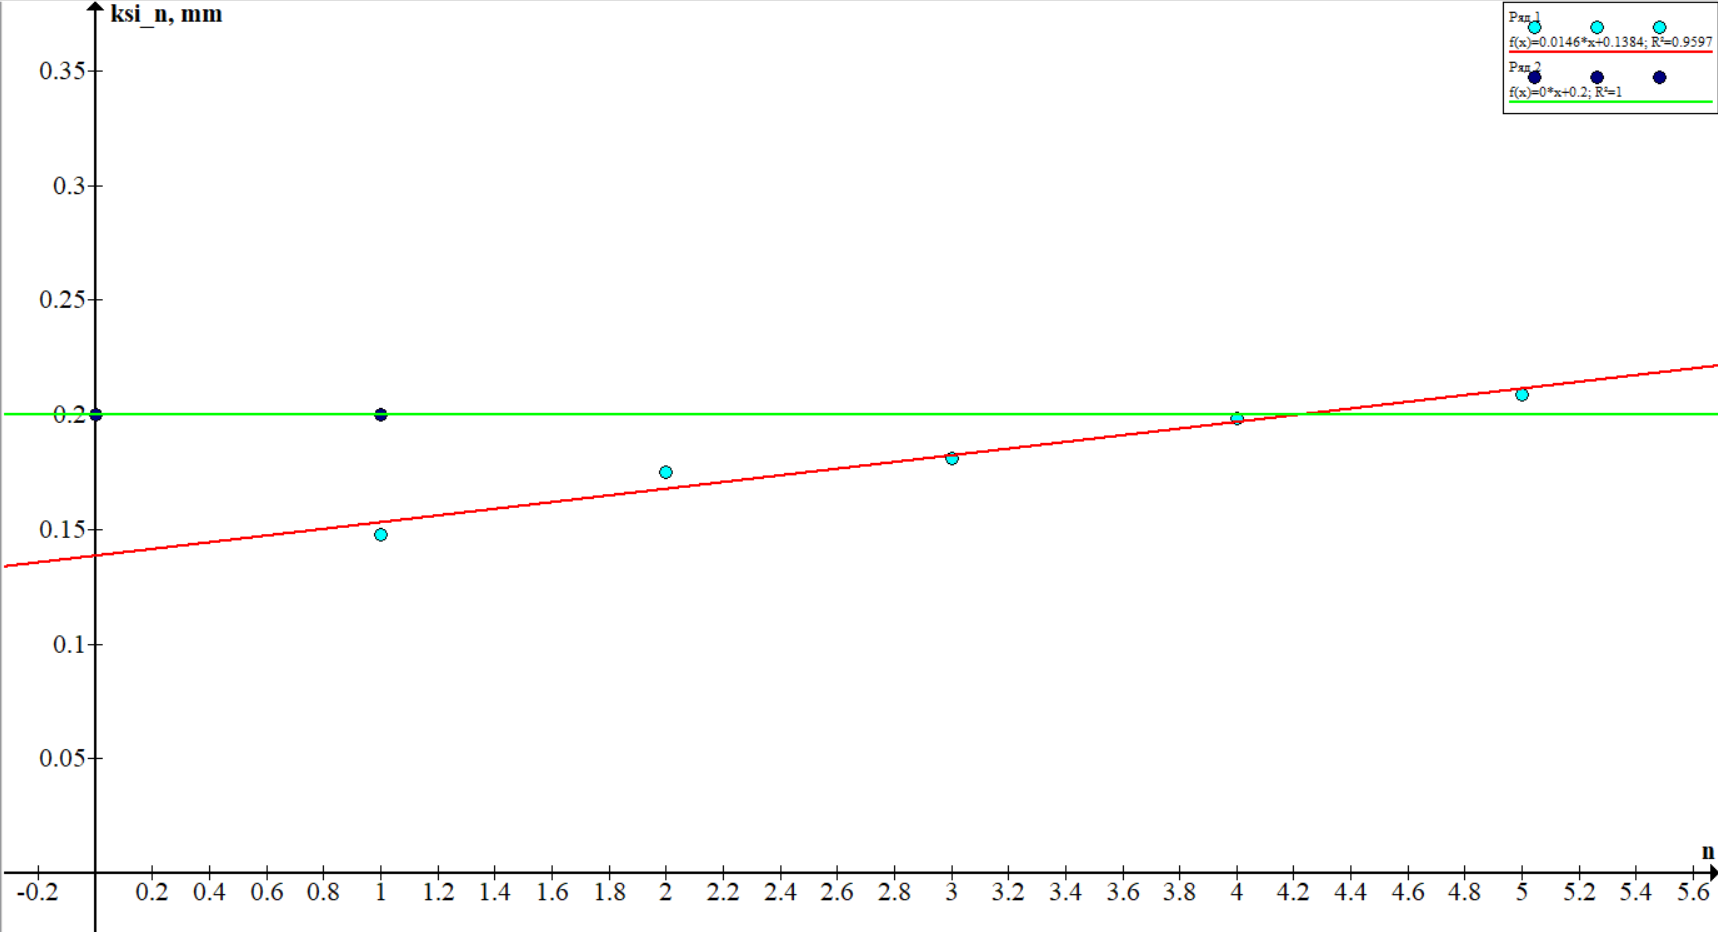
\includegraphics[scale=0.47]{pics/graph1.png}
	\caption{График зависимости суммарной ширины зон Френеля от их числа}
\end{figure}

%Таким образом, ширина примерно совпадает с шириной щели и является постоянной величиной. "<Сдвиг"> объясним неточностью в измерении нуля.  %


\section{Дифракция Фраунгофера на одной щели}

	\subsection{Экспериментальная установка}
	
	На значительном удалении от щели, когда выполнено условие $ C \ll 1 $
(то есть ширина щели становится значительно меньше ширины первой
зоны Френеля, $ b \ll \sqrt{\lambda z} $), изображение щели размывается и возникает
дифракционная картина, называемая дифракцией Фраунгофера.

Дифракцию Френеля и Фраунгофера можно наблюдать на одной
и той же установке (рис. 1). Однако при обычных размерах установки дифракция Фраунгофера возникает только при очень узких щелях.

	\begin{figure}[h!]
		\centering
		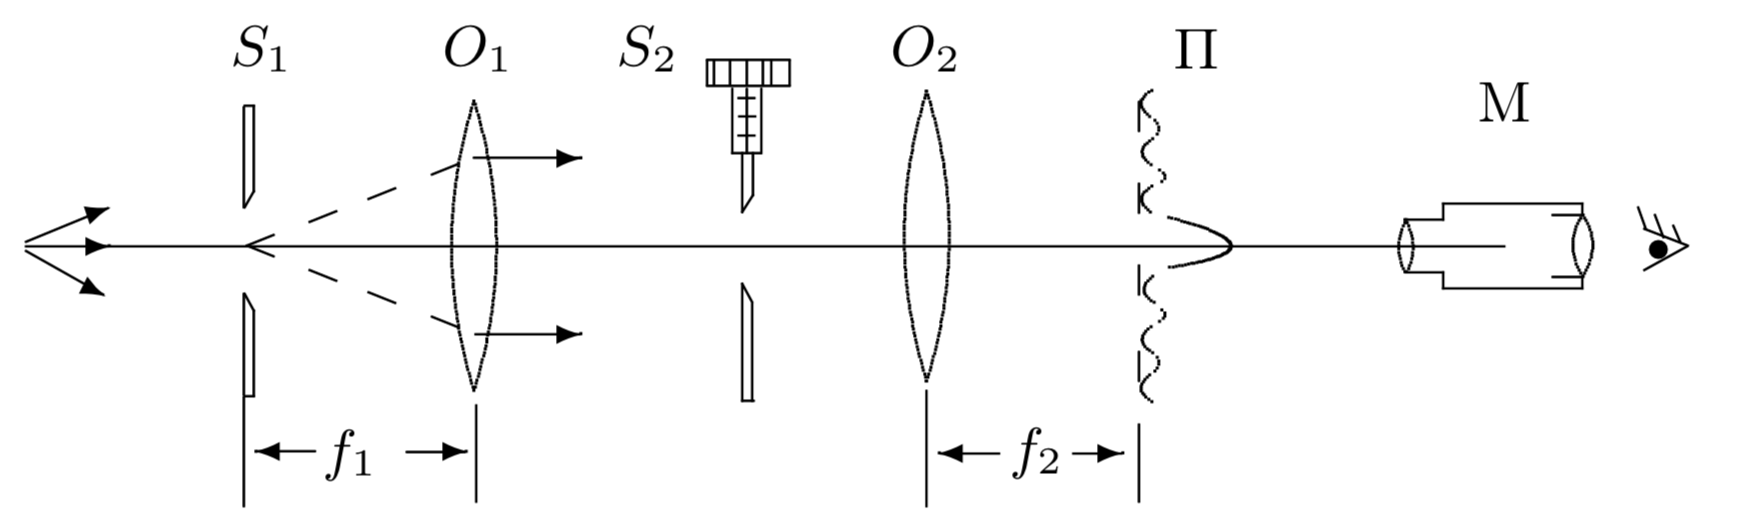
\includegraphics[width=0.8\linewidth]{pics/b.png}
		\caption{Экспериментальная установка B}
		\label{labB}
	\end{figure}

Например, при $ z \approx$ 20-40 см и $ \lambda \approx 5 \cdot $ 10-5  см получаем $b \ll 0,3$ мм. Поскольку работать с такими тонкими щелями неудобно, для наблюдения дифракции Фраунгофера к схеме, изображённой на рис. 1, добавляется объектив $ O_2  $(рис. 3).

Дифракционная картина наблюдается здесь в фокальной плоскости
объектива $ O_2 $. Каждому значению угла $ \theta $ соответствует в этой плоскости точка, отстоящая от оптической оси на расстоянии

\begin{equation}\label{x}
x = f_2 \tg \theta \approx f_2 \theta
\end{equation}

Поскольку объектив не вносит дополнительной разности хода
между интерферирующими лучами (таутохронизм), в его фокальной
плоскости наблюдается неискаженная дифракционная картина Фраунгофера. Эта картина соответствует бесконечно удалённой плоскости
наблюдения.

В центре поля зрения наблюдается дифракционный максимум (светлая полоса). При малых углах $ \theta $ положение минимумов (тёмных полос)
определяется, соотношением

\begin{equation}\label{theta_m}
\theta_m = m \dfrac{\lambda}{b}
\end{equation}

Расстояние $ x_m $ от тёмной полосы до оптической оси объектива $ O_2 $ пропорционально фокусному расстоянию $ f_2 $. Из \eqref{x} и \eqref{theta_m} следует 

\begin{equation}\label{xm}
x_m = m \dfrac{\lambda}{b} f_2
\end{equation}

Видно, что при малых углах минимумы эквидистантны, а
расстояния $ \delta x $ между минимумами обратно пропорциональны ширине $ b $ щели $ S_2 $


\subsection{Измерения и обработка результатов}

Величина щели по винту равна $ b = 0.2 \pm 0,02 $ мм. Фокусное расстояние линзы $ f_2 = 13,8 $ см.

Измерим с помощью винта поперечного перемещения микроскопа координаты $ X_m $ нескольких дифракционных минимумов. З
Результаты занесем в табл. 2 и построим график зависимости минимумов от их номеров. 

\begin{table}[h!]
	\caption{Зависимость минимумов от их номера $ m $}
	\begin{center}
		\begin{tabular}{|c|c|c|}
			\hline
			$ x_m $, кол-во делений & $ X_m $, мм & $ m $, номер минимума \\
			\hline
			0 & 0   &    -3 \\
			\hline
			15 & 0.6 &   -2 \\
            \hline
			27 & 1.08 &  -1\\
			\hline
			40 & 1.6 &    0 \\
			\hline
			53 & 2.12 &    1 \\
			\hline
			64 & 2.56 &   2\\
			\hline
			73 & 2.92 &   3 \\
			\hline
		\end{tabular}
	\end{center}
	\label{}
\end{table}

	\begin{figure}[h!]
	\label{graf_b}
	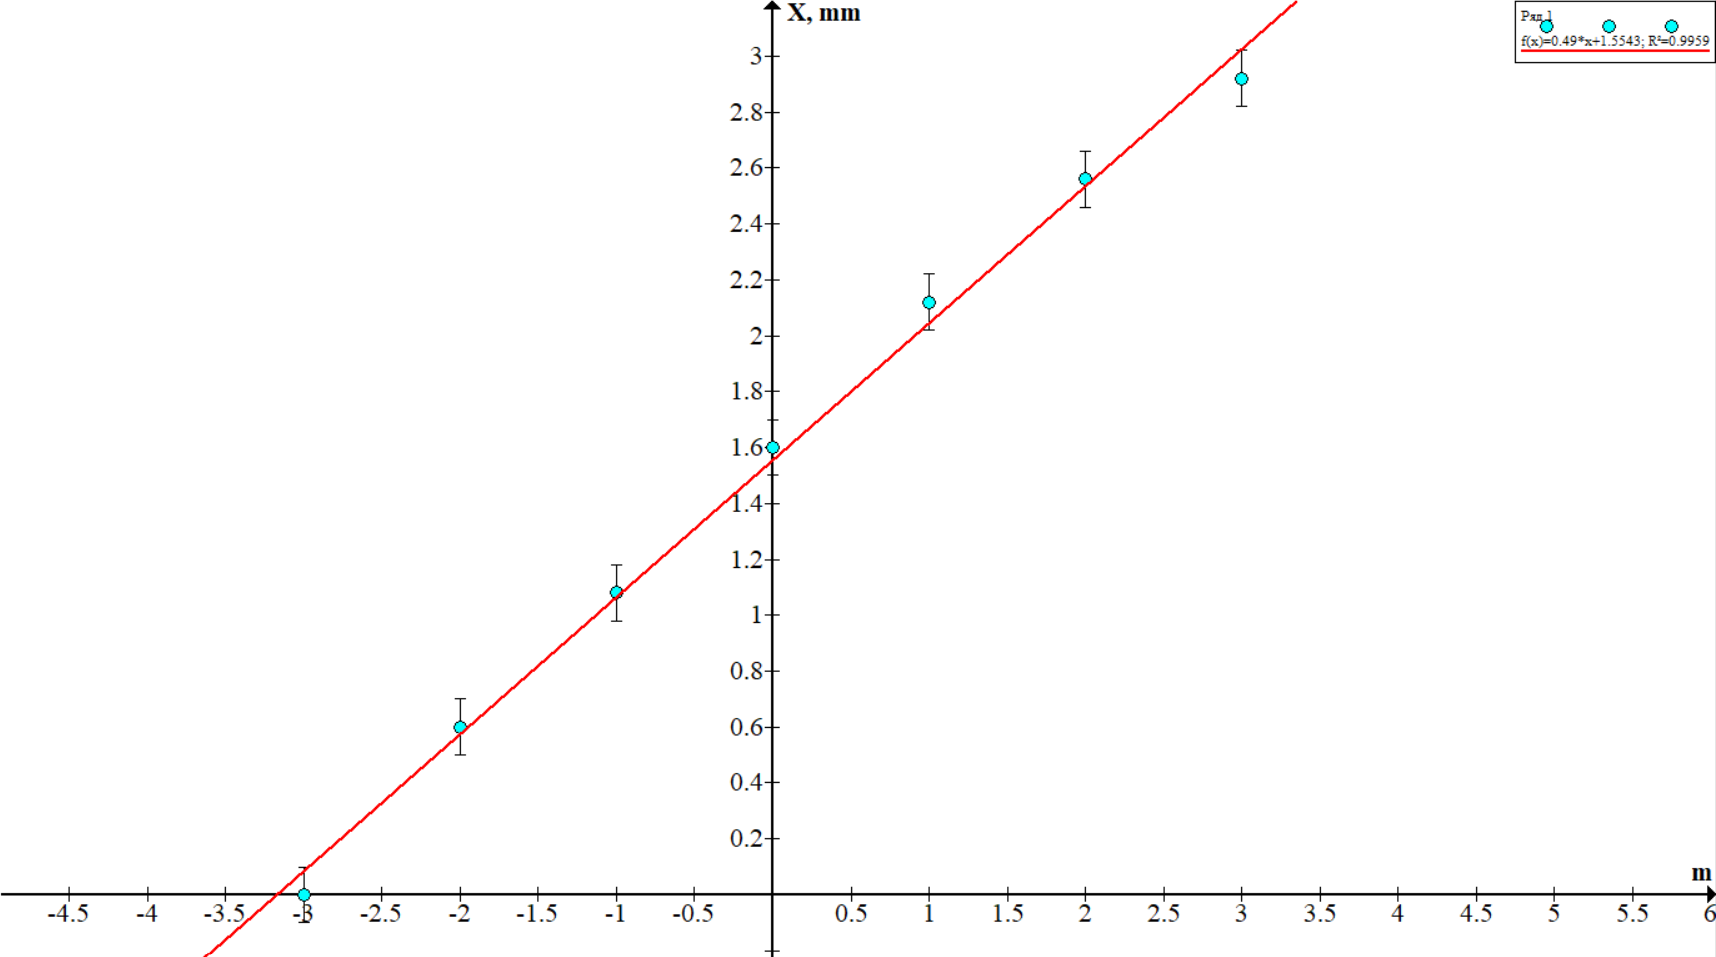
\includegraphics[scale=0.47]{pics/graph2.png}
	\caption{График зависимость $ X_m $ минимумов от их номера $ m $}
\end{figure}


Из графика получаем, что угол наклона $ a = 0.49 $ мм. Это и есть расстояние $ \Delta X $ между соседними максимумами. Из формулы \eqref{xm} мы получаем, что 

\[ a = \frac{\lambda f_2}{b_{exp}} \Rightarrow   \]
\[ b_{exp} = \frac{\lambda f_2}{a} \approx  0.15 \: \text{мм}    \]

Таким образом, наши значения для $ b $ и $ b_{exp} $ близки. 

\newpage

\section{Дифракция Фраунгофера на двух щелях}

\subsection{Экспериментальная установка}

Для наблюдения дифракции Фраунгофера на двух щелях в установке (рис. 3) следует заменить щель $ S_2 $ экраном Э с двумя щелями
(рис. 4). При этом для оценки влияния ширины входной щели на чёткость дифракционной картины вместо входной щели $ S_1 $ следует поставить щель с микрометрическим винтом. Два дифракционных изображения входной щели, одно из которых образовано лучами, прошедшими через левую, а другое --- через правую щели, накладываются друг на друга.

	\begin{figure}[h!]
		\centering
		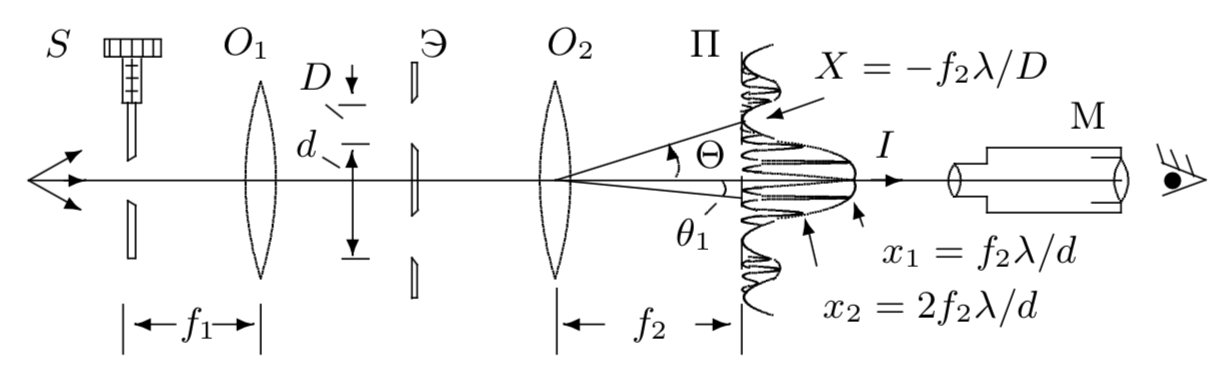
\includegraphics[width=0.8\linewidth]{pics/c.png}
		\caption{Экспериментальная установка C}
		\label{labC}
	\end{figure}

Если входная щель достаточно узка, то дифракционная картина
в плоскости П (рис. 4) подобна той, что получалась при дифракции
на одной щели (рис. 3), однако теперь вся картина испещрена рядом
дополнительных узких полос.
Угловая координата $ \theta_m $ интерференционного максимума $ m $-го порядка определяется соотношением

\begin{equation}\label{}
\theta_m = m \dfrac{\lambda}{b}
\end{equation}

где $ d $ --- расстояние между щелями. Линейное расстояние $ \delta x $ между соседними интерференционными полосами в плоскости П равно, поэтому

\begin{equation}\label{dx}
\delta x = f_2 \dfrac{\lambda}{d}
\end{equation}

На рис. 4 показано распределение интенсивности в фокальной плоскости объектива $ O_2 $. Штриховой линией (в увеличенном масштабе)
изображено распределение интенсивности при дифракции света на одиночной щели. Нетрудно оценить число n интерференционных полос,
укладывающихся в области центрального дифракционного максимума.
Согласно \eqref{xm} полная ширина главного максимума равна $ 2 f_2 \lambda /b $, где $ b $ ширина щели, отсюда

\begin{equation}\label{n}
n = \dfrac{2f_2 \lambda}{b} \dfrac{1}{\delta x} = \dfrac{2d}{b}
\end{equation}

При дифракции света на двух щелях чёткая система интерференционных полос наблюдается только при достаточно узкой ширине входной щели $ S $, которую можно рассматривать как протяжённый источник света размером $ b $. Для наблюдения интерференции необходимо, чтобы расстояние $ d $между щелями не превышало радиуса когерентности

\begin{equation}\label{}
d \ll \dfrac{\lambda}{b} f_1
\end{equation}

Здесь $ b $ --- ширина входной щели $ S $ и, следовательно, $  b/f_1 $ --- её угловая ширина. Таким образом, по размытию интерференционной картины можно оценить размер источника. Этот метод используется в звёздном интерферометре при измерении угловых размеров звёзд.

\subsection{Измерения и обработка результатов}

Получим на экране дифракционную картину и проведем измерения. Определим координаты $x_1$ и $x_2$ - координаты самых удаленных друг от друга темных полос внутри первого максимума.



 \textbf{Измерим ширину главного максимума.}
 \newline
 $  \delta x  = (x_{1} - x_{2} )= 0.048 $ мм

 Из формулы \eqref{dx} получаем \textbf{расстояние между щелями}:
 
 \[d = \dfrac{f_2 \lambda}{\delta x} = 1.17 \pm 0,04 \; \text{мм}\]
 
 \[ \sigma_d = d\cdot \frac{\sigma_{\delta x}}{\delta x}       \]
 
 \textbf{Измеренное $d_0 = $ 1.1 mm}:
\newline
 Заметим, что измеренное $d_0$ и рассчитанное $d$ неплохо близки по значению.
 
\textbf{Рассчитаем ширину щели}:
\newline
Измеренное $b_0 \approx 0.12$ \: мм.
 
 \begin{equation}\label{}
 b = \dfrac{2 f_2 \lambda}{d} = 0,121 \pm \;0,004 \: \text{мм}
 \end{equation}
 
 Аналогично замечаем, что измеренное хорошо совпадает с рассчитанным.
 
 Из формулы \eqref{n} оценим количество полос внутри главного максимума:
 
 \[ n = \frac{2d}{b} = \frac{2 \cdot 1.17}{0.26}  \approx 7 \: \text{полос}   \] 
 
И действительно, внутри главного максимума наблюдалось 7 полос.
 
 \section{Вывод}
 
 В ходе работы мы изучили два основных типа дифракции: Френеля и Фраунгофера при разных размерах щели и провели качественные наблюдения этих явлений, а также экспериментально проверили справедливость теоретических формул.  
 
 В первой части работы была получена зависимость координаты дифракционного минимума от его номера. 
 С помощью полученного угла наклона прямой удалось расчитать ширину щели. Измеренное значение неплохо совпадало с рассчитанным.
 
Во второй части была получена дифракционная картина для дифр. Фраунгофера. Вычисленные величины $d, \: b$ и их сравнение с $d_0, \: b_0$ приведено чуть выше.

\end{document}